

\begin{figure}[p]
    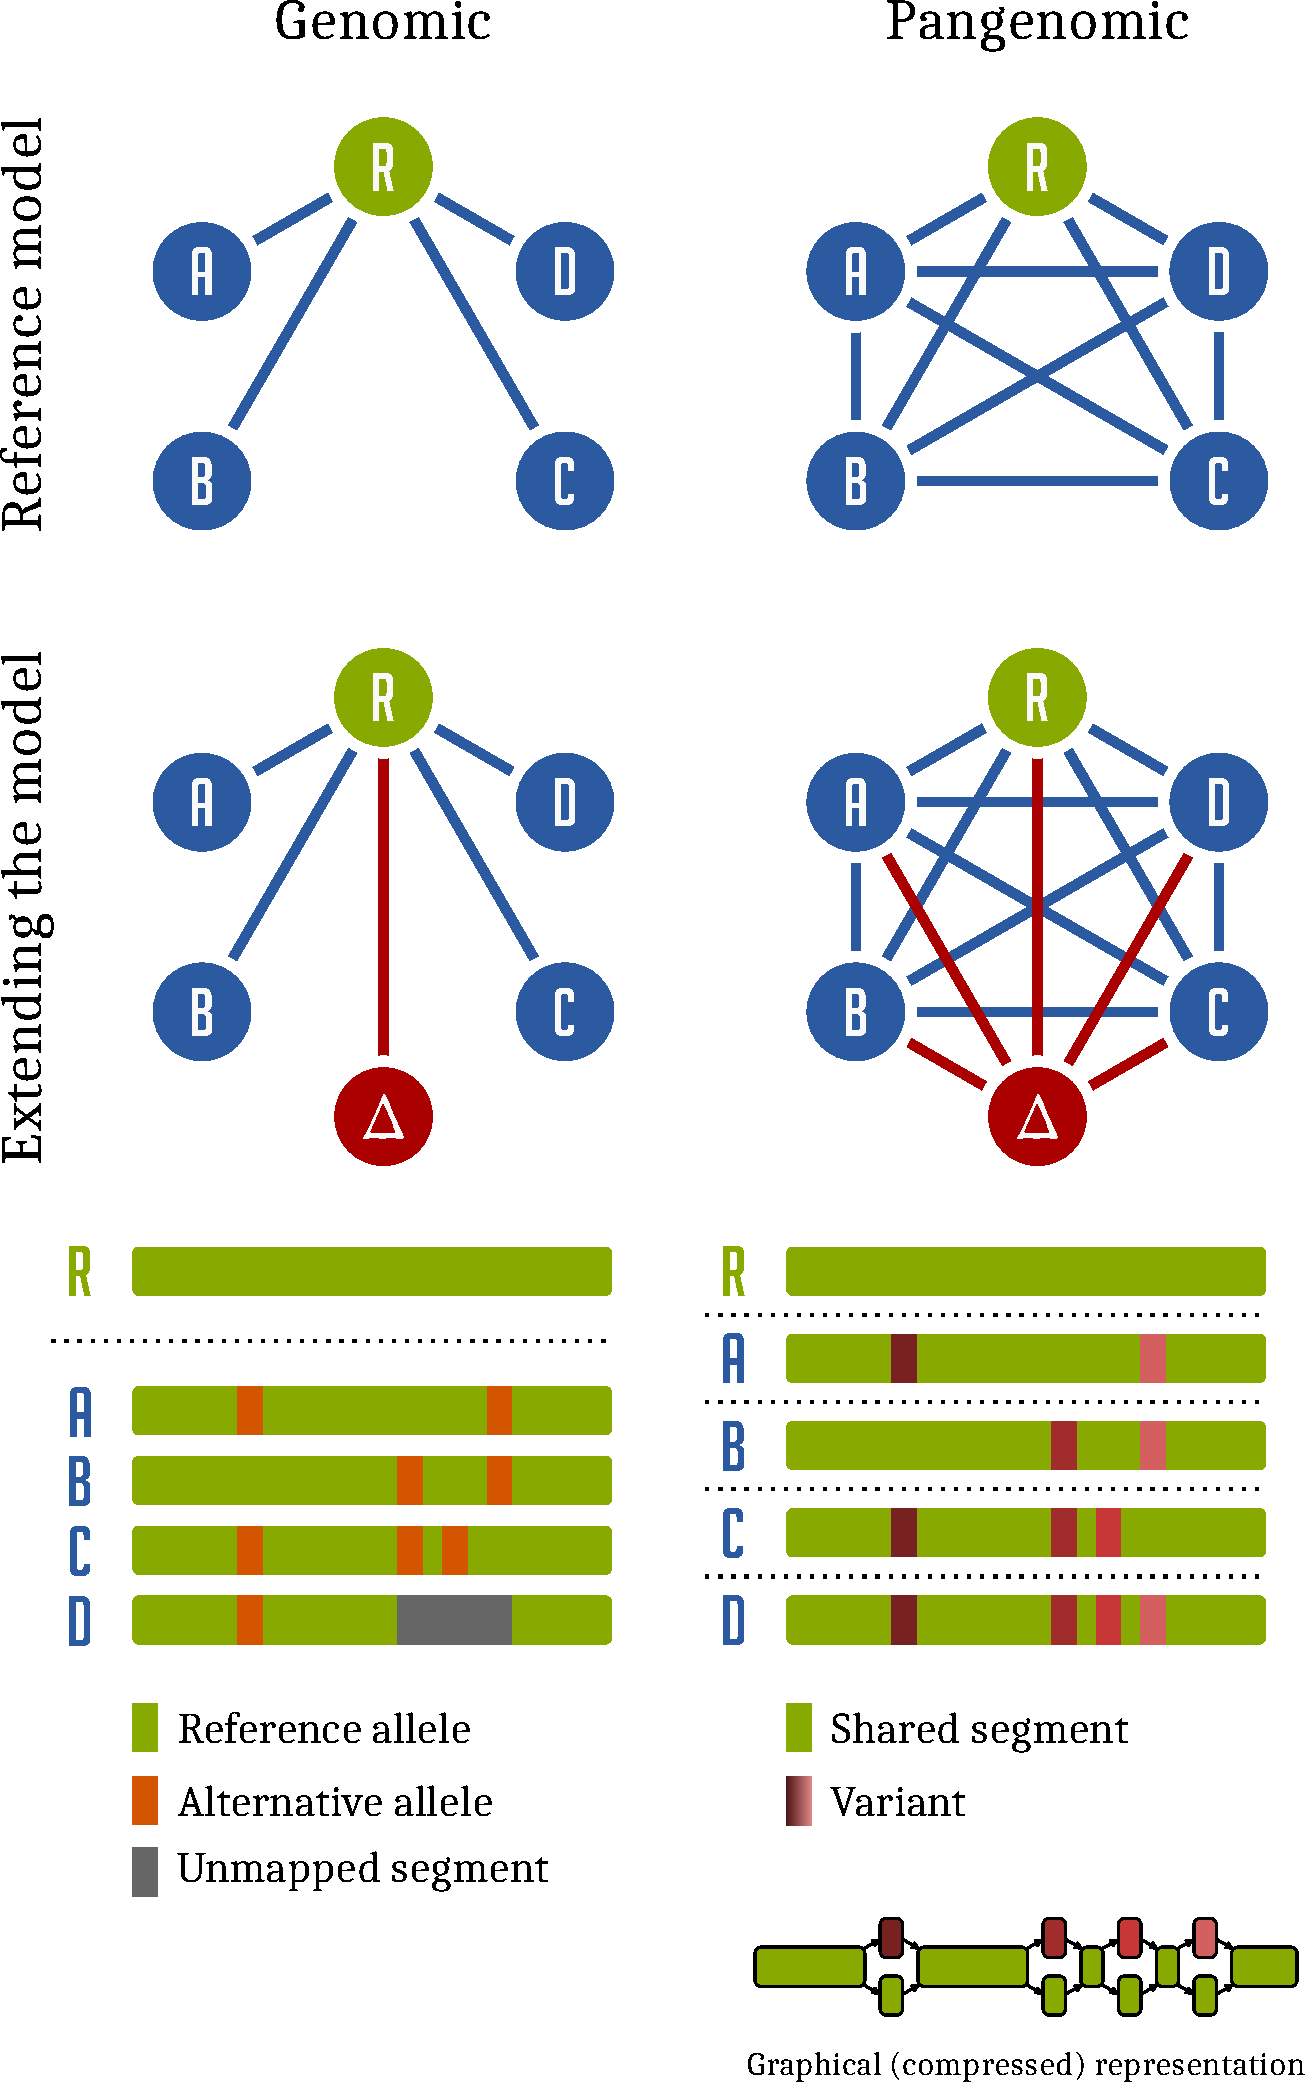
\includegraphics[width=0.8\textwidth]{figures/gen_vs_pang.pdf}
    \caption{\label{fig:genvpan} Genomic versus pangenomic sequence analysis patterns.
      %Top left: In reference based genomic analyses, all genomes ($a \ldots f$) are compared to each other via their relationship to the reference genome $R$.
      %Top right: In a pangenomic setting, we attempt to model direct relationships between all the genomes in our analysis, of which a particular reference $R$ is chosen arbitrarily.
      %Bottom left: When extending our analysis with a new genome, $\Delta$, we add it to the genomic model by comparing it to reference $R$.
      %Bottom right: In contrast, adding a new genome to a pangenomic analysis compares it directly with all other genomes in the model.
    }
\end{figure}

\begin{figure}[p]
    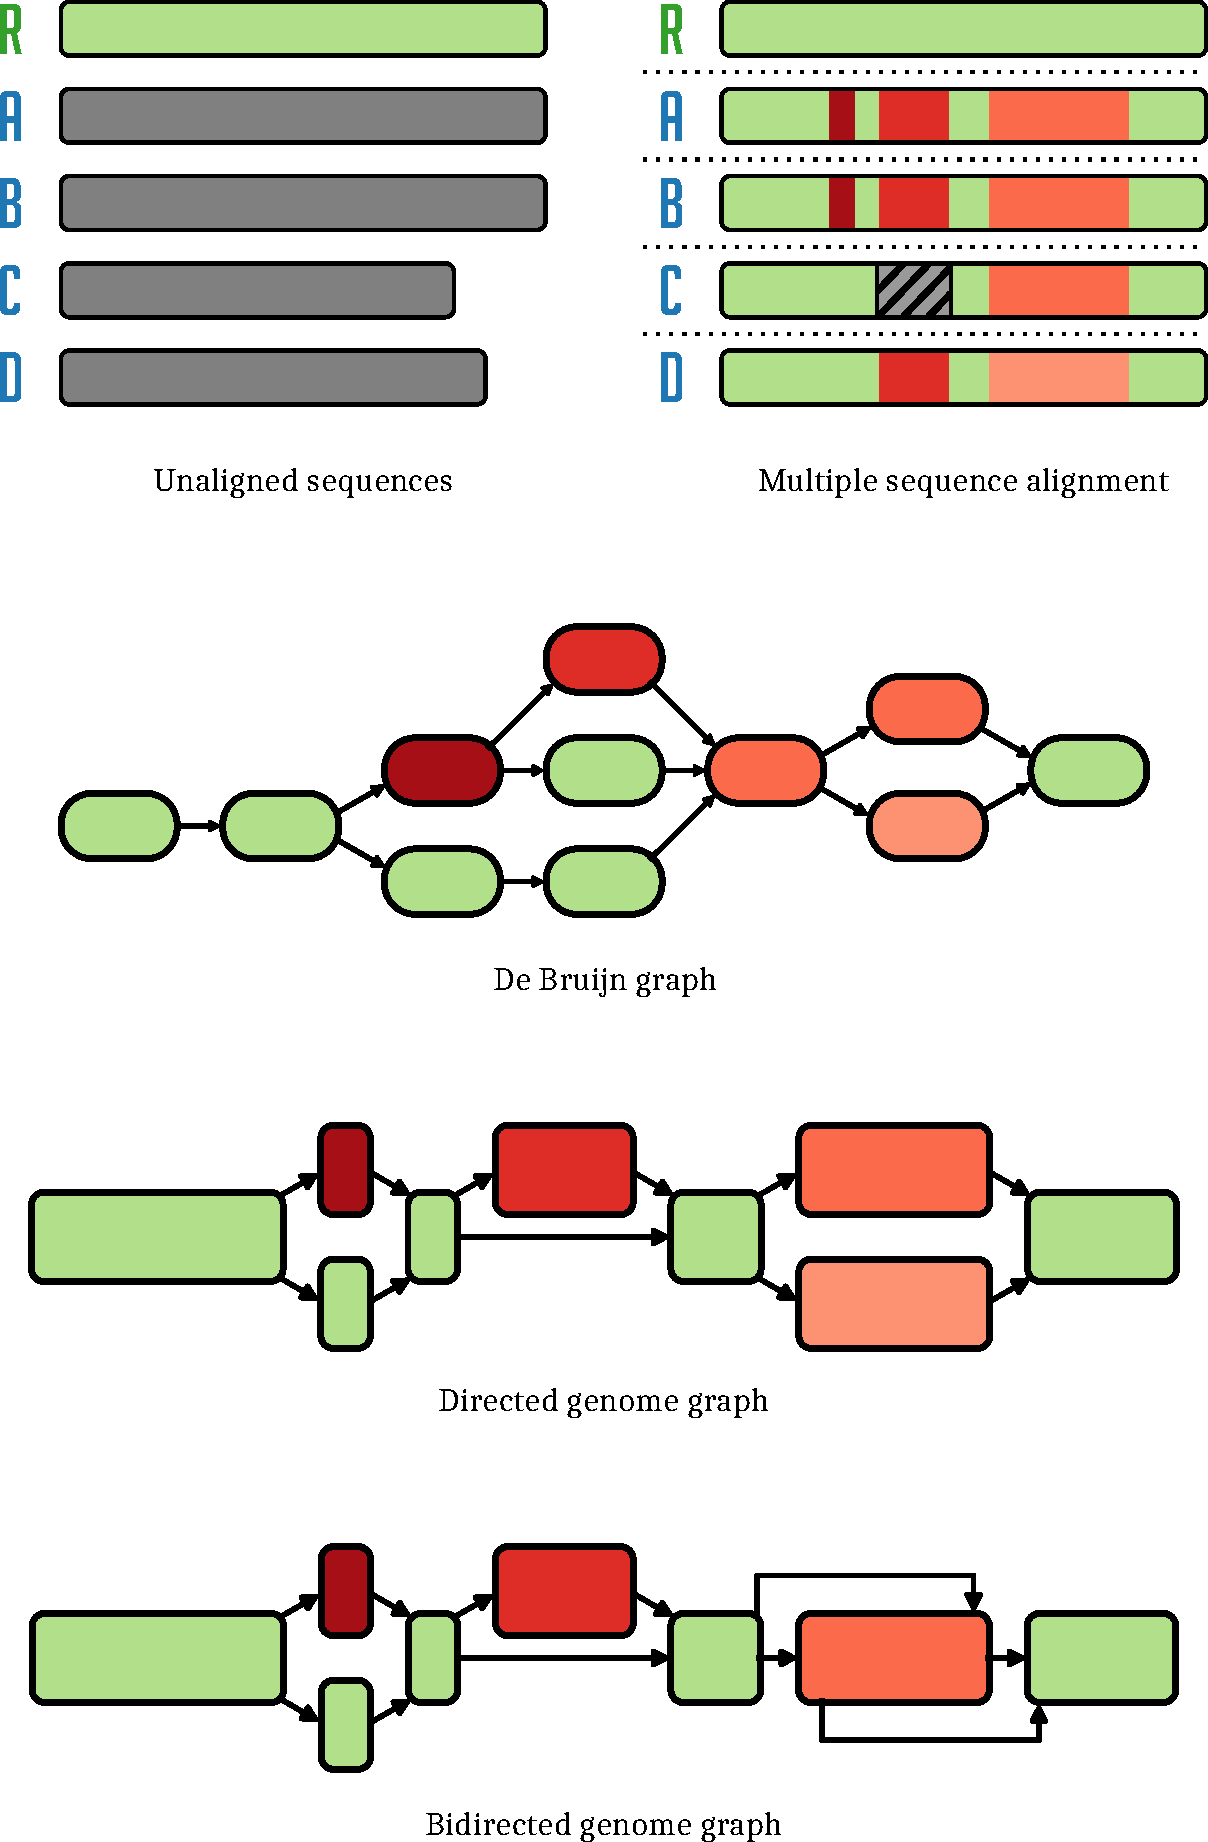
\includegraphics[width=0.9\textwidth]{figures/data_structures.pdf}
    \caption{\label{fig:models} Pangenomic models.
      A collection of sequences representing a pangenome, their alignment, a acyclic sequence graph representing the linear alignment, and a generic sequence graph including an inversion.
    }
\end{figure}

\begin{figure}[h]
    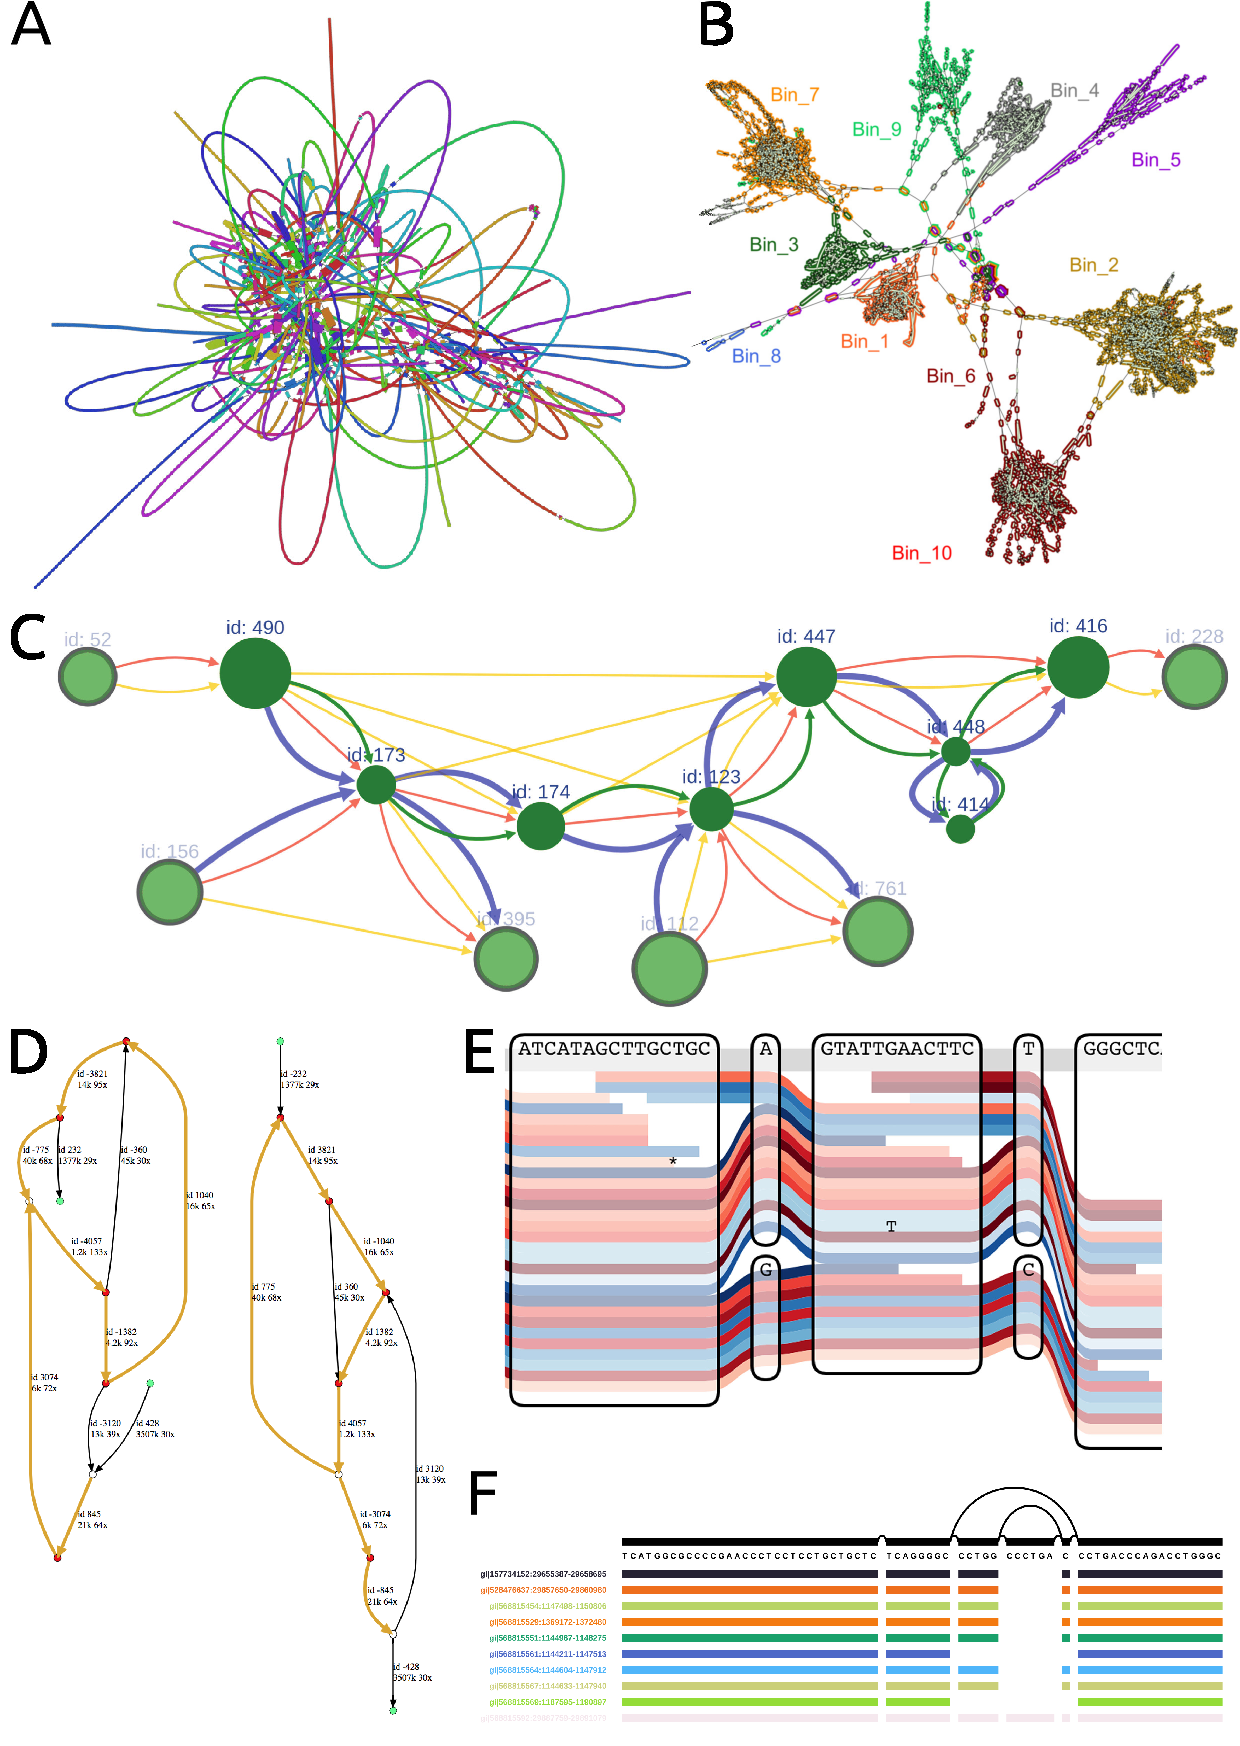
\includegraphics[width=0.9\textwidth]{figures/visualization.pdf}
    \caption{\label{fig:visualization} An overview of several approaches to visualizing assembly, scaffold, and comprehensive pangenome graphs.
\textbf{A:} Bandage, adapted from \cite{Wick_2015} supplementary section~6.
\textbf{B:} GfaViz, adapted from \cite{Gonnella_2018} supplementary figure~S4.
\textbf{C:} SGTK, adapted from \cite{Kunyavskaya_2018} figure~1.
\textbf{D:} AGB, adapted from \cite{Mikheenko_2019} supplementary figure~S3.
\textbf{E:} Sequence Tube Map, adapted from \cite{Beyer_2019} figure~2.
\textbf{F:} \texttt{vg viz}, adapted from \cite{Garrison_2019} figure~2.20.}
\end{figure}
